% !TeX root = definitions_of_asymptotic_cones.tex
\documentclass[a4paper,11pt]{jsarticle}

% 英文化
\usepackage[english]{babel}
% 数式
\usepackage{amsmath}
\usepackage{amsfonts}
\usepackage{amsthm}
\usepackage{amssymb}
\usepackage{bm}
\usepackage{mathtools}
% 画像
\usepackage[dvipdfmx]{graphicx}
% 箇条書き
\usepackage{enumitem}

% 枠付き文章
\usepackage{ascmac}

\newcommand{\QUOTEBOX}[1]{\begin{center}\fbox{\begin{minipage}{.8\textwidth}{#1}\end{minipage}}\end{center}}
\newcommand{\DEFINITION}[2]{\begin{itembox}[l]{\underline{Definition {#1} }}{#2}\end{itembox}}
\newcommand{\PROPOSITION}[2]{\begin{itembox}[l]{\underline{Proposition {#1} }}{#2}\end{itembox}}
\newcommand{\REMARK}[2]{\begin{itembox}[l]{\underline{Remark {#1} }}{#2}\end{itembox}}

\newcommand{\NaturalNumberSet}{\mathbb{N}}
\newcommand{\RealNumberSet}{\mathbb{R}}
\newcommand{\NDemenstionalRealEuclidianSpace}{\mathbb{R}^n}

\newcommand{\SuchThat}{\:\text{s.t.}\:}



\SetLabelAlign{Center}{\hfil#1\hfil}
\SetLabelAlign{CenterWithParen}{\hfil(\makebox[1.0em]{#1})\hfil}
\SetLabelAlign{CenterWithParen2}{\hfil(\makebox[1.5em]{#1})\hfil}


\renewcommand{\theenumi}{\roman{enumi}}
\renewcommand{\labelenumi}{(\theenumi)}
\renewcommand{\theenumii}{\theenumi-\alph{enumii}}
\renewcommand{\labelenumii}{(\theenumii)}

\begin{document}

\title{
  2 Asymptotic Cones and Functions \\
  \large 2.1 Definition of Asymptotic Cones}
\author{Ryota Iwamoto}
\date{\today}
\maketitle

We use the book; Asymptotic Cones and Functions in Optimization and Variational Inequalities (author: A.AUSLENDER and M.TEBOULLE), pp.25-31.

\QUOTEBOX{
  The set of natural numbers is denoted by $\NaturalNumberSet$, so that $k \in \NaturalNumberSet$ means $k = 1,2, \dots .$ A sequence $\{x_k\}_{k \in \NaturalNumberSet}$ or simply $\{x_k\}$ in $\NDemenstionalRealEuclidianSpace$ is said to converge to $x$ if $\left\lVert x_k - x\right\rVert \rightarrow 0$ as $k \rightarrow \infty$, and this will be indicated by the notation $x_k \rightarrow x$ or $x = \lim_{k \to \infty} x_k$. We say that $x$ is a cluster point of $\{x_k\}$ if some subsequence converge to $x$. Recall that every bounded sequence in $\NDemenstionalRealEuclidianSpace$ converges to $x$ if and only if it is bounded and has $x$ as its unique cluster point.

  Let $\{x_k\}$ be a sequence in $\NDemenstionalRealEuclidianSpace$. We are interested in knowing how to handle convergence properties, we are led to consider direction $d_k \coloneqq x_k\left\lVert x_k\right\rVert^{-1}$ with $x_k \neq 0$, $k \in \NaturalNumberSet$. From classical analysis, the Bolzano-Weierstrass theorem implies that we can extract a convergent subsequence $d = \lim_{k \in K} d_k$, $K \subset \NaturalNumberSet$, with $d \neq 0$. Now suppose that the sequence $\{x_k\} \subset \NDemenstionalRealEuclidianSpace$ is such that $\left\lVert x_k \right\rVert \rightarrow + \infty$. Then
  \begin{equation}
    \exists t_k \coloneqq \left\lVert x_k \right\rVert, k \in K \subset \NaturalNumberSet, \text{ such that } \lim_{k \in K} t_k = + \infty \:\text{and}\: \lim_{k \in K} \frac{x_k}{t_k} = d. \notag
  \end{equation}
  This leads us to introduce the following concepts.
}

\DEFINITION{2.1.1}{
  A sequence $\{x_k\} \subset \RealNumberSet$ is said to converge to a direction $d \in \NDemenstionalRealEuclidianSpace$ if
  \begin{equation}
    \exists \{t_k\}, \:with\: t_k \rightarrow + \infty \:\text{ such that }\: \lim_{k \to \infty} \frac{x_k}{t_k} = d. \notag
  \end{equation}
}

\DEFINITION{2.1.2}{
  Let $C$ be a nonempty set in $\NDemenstionalRealEuclidianSpace$. Then the asymptotic cone of the set $C$, denoted by $C_{\infty}$, is the set of vectors $d \in \NDemenstionalRealEuclidianSpace$ that are limits in direction of the sequences $\{x_k\} \subset C$, namely
  \begin{equation}
    C_{\infty} = \{d \in \NDemenstionalRealEuclidianSpace \:|\: \exists t_k \rightarrow + \infty , \exists x_k \in C \:\text{ with }\: \lim_{k \to \infty} \frac{x_k}{t_k} = d \}. \notag
  \end{equation}
}

\QUOTEBOX{
  From the definition we immediately deduce the following elementary facts.
}

\PROPOSITION{2.1.1}{
  Let $C \subset \NDemenstionalRealEuclidianSpace$ be nonempty. Then:
  \begin{enumerate}[label=\roman*,align=CenterWithParen]
    \item $C_{\infty}$ is a closed cone.
    \item $(\text{cl}\:C)_{\infty} = C_{\infty}$.
    \item If $C$ is a cone, then $C_{\infty} = \text{cl}\:C$.
  \end{enumerate}
}

\begin{proof}
  We will prove each part separately.
  \begin{enumerate}[label=\roman*,align=CenterWithParen]
    \item $C_{\infty}$ is a closed cone.

      We need to show two propositions: (i-a) $C_{\infty}$ is a cone and (i-b) $C_{\infty}$ is a closed set.

      \begin{enumerate}[label=i-\alph*,align=CenterWithParen]
        \item We show that $C_{\infty}$ is a cone, that is, $\forall \alpha \geq 0, d \in C_{\infty}, \alpha d \in C_{\infty}$.

        Since $0$ is a element of $C_{\infty}$, it is clear in the case of $\alpha = 0$.

        ($\because$ Since $C$ is nonempty, we can take a element $x_0$ from $C$. In addition we take a sequence $\{t_k\}_{k=1}^{\infty}$ with $t_k \rightarrow + \infty$ as $k \rightarrow \infty$. Of course this sequence exists, for example $t_k \coloneqq k$. By using $t_k \coloneqq k$ and $x_k \coloneqq x_0$, we can obtain $0$ as the limit. Hence $0$ is a element of $C_{\infty}$.)

        Also we consider the other case $\alpha > 0$. To prove that $C_{\infty}$ is a cone, we take a any direction $d$ from $C_{\infty}$. Since d is a element of $C_{\infty}$,

        \begin{equation}
          \exists t_k \rightarrow + \infty , \exists x_k \in C \:\text{ with }\: \lim_{k \to \infty} \frac{x_k}{t_k} = d. \notag
        \end{equation}

        Then we define a sequence $\{t'_k\}_{k=1}^{\infty} \coloneqq \frac{t_k}{\alpha}$, exactly whose limit becomes $+\infty$ as $k \rightarrow \infty$. Accordingly there exist $t'_k \rightarrow + \infty$ and $x_k \in C$ with

        \begin{equation}
          \lim_{k \to \infty} \frac{x_k}{t'_k} = \lim_{k \to \infty} \alpha \cdot \frac{x_k}{t_k} = \alpha d. \notag
        \end{equation}

        This means $d \in C_{\infty}$.

        By these results, we can get $\forall \alpha \geq 0, d \in C_{\infty}, \alpha d \in C_{\infty}$.

        Therefore $C_{\infty}$ is a cone.

        \item We show that $C_{\infty}$ is a closed set. In order to prove closeness, we consider convergency of a sequence in $C_{\infty}$. First we take a sequence $\{d_k\}_{k=1}^{\infty} \subset C_{\infty}$ with $d_k \rightarrow d$ as $k \rightarrow \infty$ for some $d$. To obtain $d \in C_{\infty}$, we need two sequences like $\{t_n\}_{n=1}^{\infty}$ with $t_n \rightarrow \infty$ as $n \rightarrow \infty$ and $\{x_n\}_{n=1}^{\infty}$ where $\frac{x_n}{t_n} \rightarrow d$ as $n \rightarrow \infty$.

        Since $d_k \rightarrow d$ and ${t_k^m}^{-1} \cdot x_k^m \rightarrow d_k$ as $m \rightarrow \infty$ for each $k \in \NaturalNumberSet$,

        \begin{equation}
          \begin{split}
            \forall n &\in \NaturalNumberSet, \exists k(n) \in \NaturalNumberSet \SuchThat \forall j \geq k(n), ||d_j -d|| < \frac{1}{n}, \text{and} \\
            \forall k &\in \NaturalNumberSet (1 \leq k \leq k(n)), \exists m(n,k) \in \NaturalNumberSet \SuchThat \forall m \geq m(n,k), ||\frac{x_k^m}{t_k^m} -d_k|| < \frac{1}{n}. \notag
          \end{split}
        \end{equation}

        Now we can rearrange

        \begin{equation}
          \begin{split}
          k(n) &\coloneqq \max\{k(n-1),k(n)\} + n \:\text{and}\: \\
          m(n) &\coloneqq \max_{1 \leq k \leq k(n)}\{m(n,k)\} + n \notag
          \end{split}
        \end{equation}

        as sequences of $n \in \NaturalNumberSet$. Then it holds that $k(1) \leq k(2) \leq \ldots$ and $m(1) \leq m(2) \leq \ldots$.

        Let's define

        \begin{equation}
          \begin{split}
            t_n &\coloneqq t_{k(n)}^{m(n)}, \:\text{and}\: \\
            x_n &\coloneqq x_{k(n)}^{m(n)}. \notag
          \end{split}
        \end{equation}

        Also we can find that

        \begin{equation}
          \begin{split}
            t_n &\rightarrow \infty \:\text{as}\: n \rightarrow \infty, \\
            x_n &\in C, \:\text{and}\: \\
            \frac{x_n}{t_n} &= \frac{x_{k(n)}^{m(n)}}{t_{k(n)}^{m(n)}}. \notag
          \end{split}
        \end{equation}

        Hence we get for each $n \in \NaturalNumberSet$

        \begin{equation}
          0 \leq \left\lVert \frac{x_n}{t_n} - d\right\rVert \leq \left\lVert \frac{x_{k(n)}^{m(n)}}{t_{k(n)}^{m(n)}} - d_{k(n)}\right\rVert + \left\lVert d_{k(n)} -d \right\rVert< \frac{1}{2n} \rightarrow 0 \notag
        \end{equation}

        as $n \rightarrow \infty$.

        Thus $d \in C_{\infty}$, that is, $C_{\infty}$ is a closed set.
      \end{enumerate}
      Then (i)'s proof is completed.
    \item $(\text{cl}\:C)_{\infty} = C_{\infty}$.

    We need to show two relations: (ii-a) $(\text{cl}\:C)_{\infty} \supset C_{\infty}$ (ii-b) $(\text{cl}\:C)_{\infty} \subset C_{\infty}$.

      \begin{enumerate}[label=ii-\alph*,align=CenterWithParen2]
        \item We show that $C_{\infty}$ is included in $(\text{cl}\:C)_{\infty}$. However it is clear from the definition of asymptotic cone.

        \item We show that $(\text{cl}\:C)_{\infty} \subset C_{\infty}$. Like (i-b), we'll show that.

      \end{enumerate}
      Then (ii)'s proof is also completed.
    \item If $C$ is a cone, then $C_{\infty} = \text{cl}\:C$.

    We need to show two relations: (iii-a) $C_{\infty} \subset \text{cl}\:C$ and (iii-b) $C_{\infty} \supset  \text{cl}\:C$.

    \begin{enumerate}[label=iii-\alph*,align=CenterWithParen2]
      \item We take any direction $d \in C_{\infty}$ which satisfies

      \begin{equation}
        \exists t_k \rightarrow + \infty , \exists x_k \in C \:\text{ with }\: \lim_{k \to \infty} \frac{x_k}{t_k} = d. \notag
      \end{equation}

      Let $d_k \coloneqq \frac{x_k}{t_k}$ (with $d_k \rightarrow d$ as $k \rightarrow \infty$). Since $C$ is a cone,

      \begin{equation}
        d_k = \frac{1}{t_k} \cdot x_k \in C. \notag
      \end{equation}

      Due to $d_k \in C$, the limit of $d_k$ is a element of $\text{cl}\:C$, i.e., $d \in \text{cl}\:C$.

      Therefore $C_{\infty} \subset \text{cl}\:C$.

      \item We take any $d \in \text{cl}\:C$ and show $d \in C_{\infty}$, that is,

      \begin{equation}
        \exists t_k \rightarrow + \infty , \exists x_k \in C \:\text{ with }\: \lim_{k \to \infty} \frac{x_k}{t_k} = d. \notag
      \end{equation}

      By $d \in \text{cl}\:C$,

      \begin{equation}
        \exists \{d_k\}_{k=1}^{\infty} \in C \:\text{with}\: d_k \rightarrow d \:\text{as}\: k \rightarrow \infty, \notag
      \end{equation}

      in other words,

      \begin{equation}
        \lim_{k \to \infty} d_k = d. \notag
      \end{equation}

      We define $y_k = k \cdot d_k$ and $s_k = k$ for each $k$. Since $d_k \in C$ and $C$ is a cone, $y_k$ is also a element of $C$.

      There exist $\{s_k\}_{k=1}^{\infty}$ with $s_k \rightarrow \infty$ as $k \rightarrow \infty$ and $\{y_k\}_{k=1}^{\infty} \subset C$ such that

      \begin{equation}
        \lim_{k \to \infty} \frac{y_k}{s_k} = \lim_{k \to \infty} d_k = d. \notag
      \end{equation}

      As $d$ is a element of $C_{\infty}$, therefore $C_{\infty} \supset  \text{cl}\:C$.

    \end{enumerate}

  \end{enumerate}
\end{proof}

\QUOTEBOX{
  The importance of the asymptotic cone is revealed by the following key property, which is a immediate consequence of its definition.
}

\PROPOSITION{2.1.2}{
  A set $C \subset \NDemenstionalRealEuclidianSpace$ is bounded if and only if $C_{\infty} = \{0\}$.
}

\begin{proof}
  We show that:

  \begin{enumerate}[label=\roman*,align=CenterWithParen]
    \item a set $C \subset \NDemenstionalRealEuclidianSpace$ is bounded $\Rightarrow $ $C_{\infty} = \{0\}$, and
    \item a set $C \subset \NDemenstionalRealEuclidianSpace$ is unbounded $\Rightarrow $ $C_{\infty} \ne \{0\}$.
  \end{enumerate}

  \begin{enumerate}[label=\roman*,align=CenterWithParen]
    \item By Proposition 2.1.1 (i), $0 \in C_{\infty}$. Also, by the assumption $C$ is bounded,

    \begin{equation}
      \exists r > 0, \forall x_k \in C \:\text{where}\: k \in \NaturalNumberSet,  \left\lVert x_k \right\rVert \leq r. \notag
    \end{equation}

    For any sequence $\{t_k\}_{k=1}^{\infty}$ such that $t_k \rightarrow \infty$ as $k \rightarrow \infty$,

    \begin{equation}
      \lim_{k \to \infty} \frac{x_k}{t_k} = 0. \notag
    \end{equation}

    Thus the limit becomes only 0 for any $\{x_k\}_{k=1}^{\infty} \subset C$ and $\{t_k\}_{k=1}^{\infty}$ with $t_k \rightarrow \infty$ as $k \rightarrow \infty$.

    Therefore if $C$ is bounded then $C_{\infty} = \{0\}$.

    \item If $C$ is unbounded, then there exists a sequence $\{x_k\} \subset C$ with $x_k \ne 0$, $\forall k \in \NaturalNumberSet$, such that $t_k \coloneqq \left\lVert t_k \right\rVert \rightarrow \infty$ and thus the vectors $d_k = t_k^{-1} x_k \in \{ d \:\colon\: \left\lVert d\right\rVert = 1 \}$.

    By the Bolzano-Weierstrass, we can extract a subsequence of $\{d_k\}$ such that $\lim_{k \in K} d_k = d$, $K \subset \NaturalNumberSet$, and with $\left\lVert d \right\rVert = 1$. This nonzero vector $d$ is an element of $C_{\infty}$ by Definition 2.1.2, a contradiction.
  \end{enumerate}
\end{proof}

Figure:

Why do we take a subsequence of $\{d_k\}$?

\begin{center}
  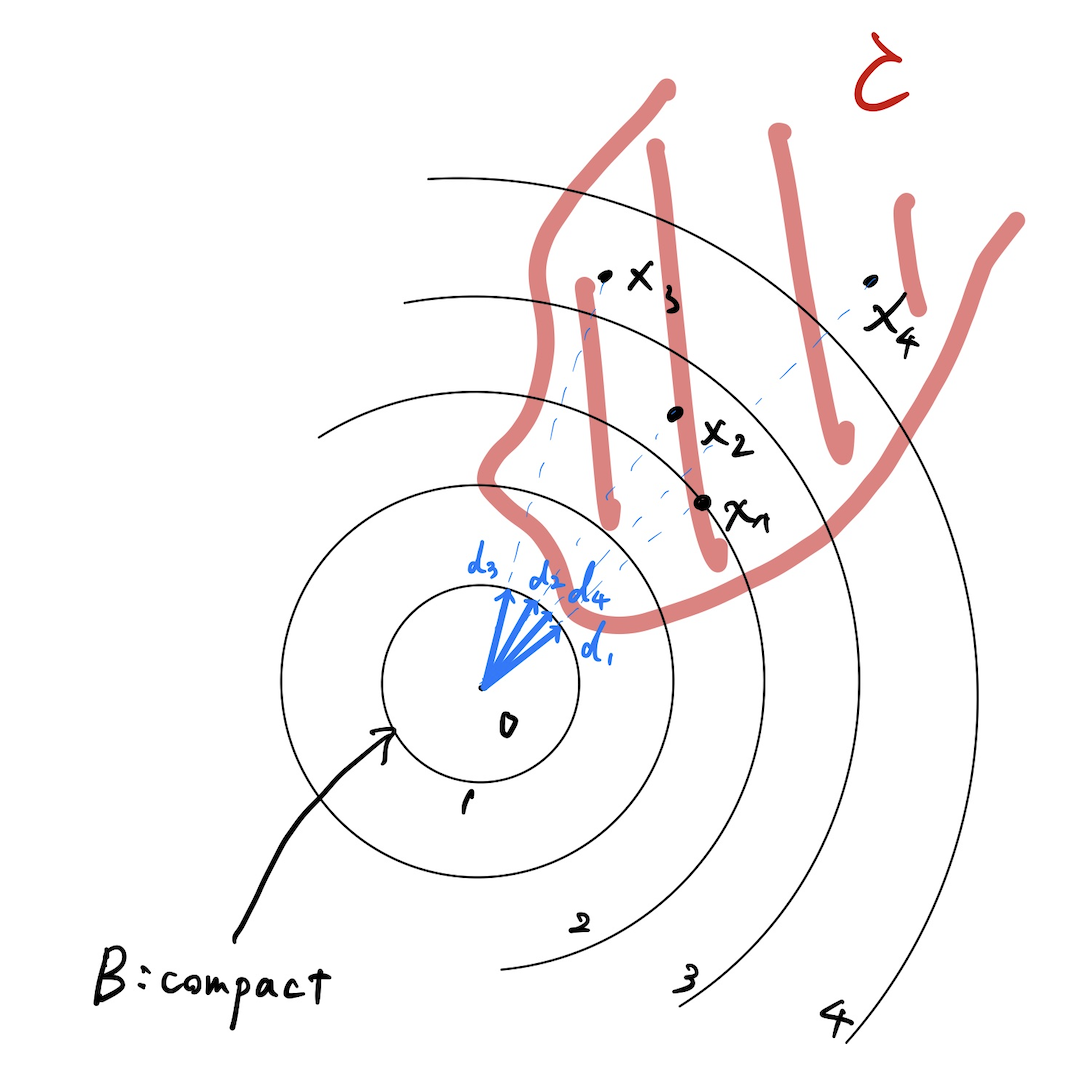
\includegraphics[width=8cm]{figures/asymptotic_cones_in_the_case_of_unbounded.png}
\end{center}

\QUOTEBOX{
  Associated with the asymptotic cone $C_{\infty}$ is the following related concept, which will help us in simplifying the definition of $C_{\infty}$ in the particular case where $C \subset \NDemenstionalRealEuclidianSpace$ is assumed convex.
}

\DEFINITION{2.1.3}{
  Let $C \subset \NDemenstionalRealEuclidianSpace$ be nonempty and define
  \begin{equation}
    C_{\infty}^1 = \{d \in \NDemenstionalRealEuclidianSpace \:|\: \forall t_k \rightarrow + \infty , \exists x_k \in C \:\text{ with }\: \lim_{k \to \infty} \frac{x_k}{t_k} = d \}. \notag
  \end{equation}
  We say that C is asymptotically regular if $C_{\infty} = C_{\infty}^1$.
}

\PROPOSITION{2.1.3}{
  Let $C$ be a nonempty convex set in $\NDemenstionalRealEuclidianSpace$. Then $C$ is asymptotically regular.
}

\begin{proof}
  The inclusion $C_{\infty}^{1} \subset C_{\infty}$ clearly holds from the definition of $C_{\infty}^{1}$ and $C_{\infty}$, respectively. Let $d \in C_{\infty}$. Then $\exists \{x_k\} \in C$, $\exists s_k \rightarrow \infty$ such that $d = \lim_{k \to \infty} s_k^{-1} x_k$. Let $x \in C$ and define $d_k = s_k^{-1}(x_k - x)$. Then we have

  \begin{equation}
    d = \lim_{k \to \infty} d_k, x + s_k d_k \in C. \notag
  \end{equation}

  $\because$ $x_k = x + s_k d_k \in C$.

  Now note that an arbitrary sequence such that $\lim_{k \to \infty} t_k = +\infty$. For any fixed $m \in \NaturalNumberSet$, there exists $k(m)$ with $\lim_{m \to \infty} k(m) = +\infty$ such that $t_m \leq s_{k(m)}$, and since $C$ is convex, we have $x'_m \coloneqq x + t_m d_{m(k)} \in C$. Hence, $d = \lim_{m \to \infty} t_m^{-1} x'_m$, showing that $d \in C_{\infty}^1$.

\end{proof}

Figure:

Why should we consider $k(m)$ with $\lim_{m \to \infty} k(m) = +\infty$ such that $t_m \leq s_{k(m)}$?

If $\{s_k\} = 1,2,3,7,8,9,13, \cdots$ and $\{t_k\} = 1,3,4,6,8,10,11, \cdots$, then we can get

\begin{equation}
  \{k(m)\} = 1,3,4,5,6,6, \cdots. \notag
\end{equation}

\begin{center}
  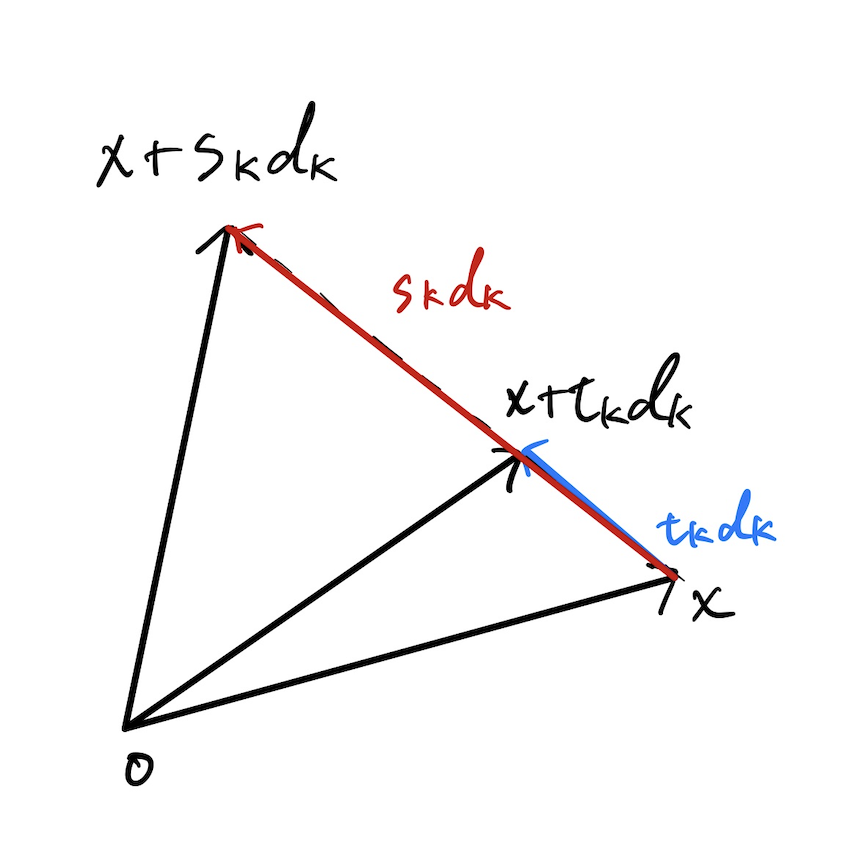
\includegraphics[width=5cm]{figures/asymptotically_regular_associated_with_convex.png}
\end{center}

\QUOTEBOX{
  We note that a set can be nonconvex, yet asymptotically regular Indeed, consider, for example, sets definition by $C \coloneqq S + K$, with $S$ compact and $K$ a closed convex cone. Then clearly $C$ is not necessarily convex, but it can be easily seen that $C_{\infty} = C_{\infty}^1$.
}


\begin{figure}[htbp]
  \begin{minipage}{0.3\hsize}
    \begin{center}
      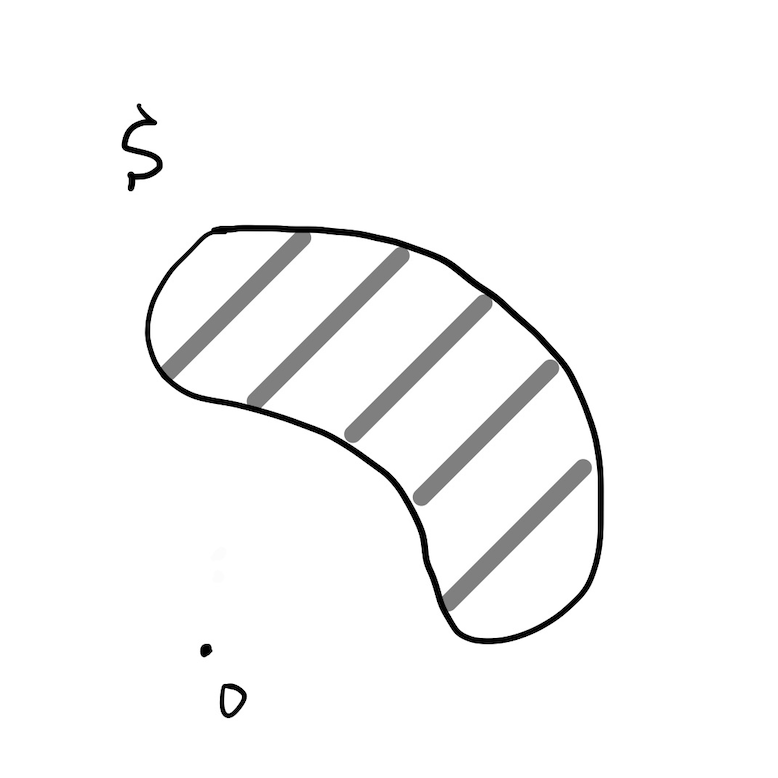
\includegraphics[keepaspectratio, width=40mm]{figures/not_convex_but_asymptotically_regular_1.png}
    \end{center}
    \caption{$S$:compact}
    \label{fig:one}
  \end{minipage}
  \begin{minipage}{0.3\hsize}
    \begin{center}
      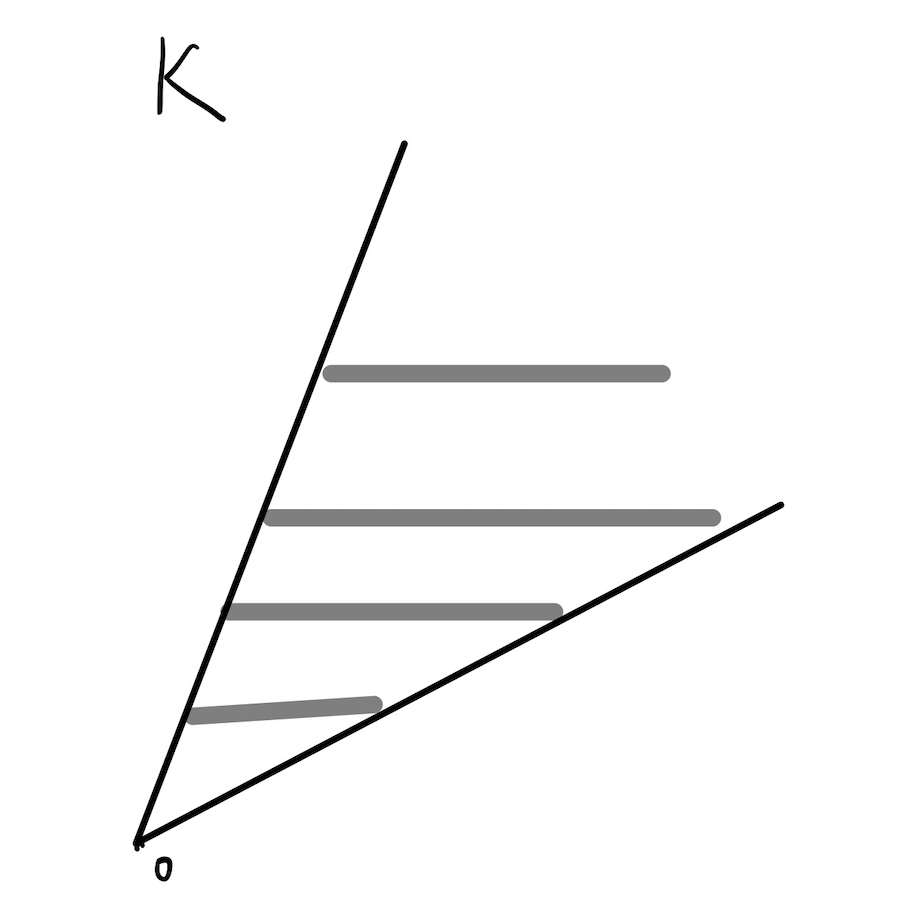
\includegraphics[keepaspectratio, width=40mm]{figures/not_convex_but_asymptotically_regular_2.png}
    \end{center}
    \caption{$K$:closed convex cone}
    \label{fig:two}
  \end{minipage}
  \begin{minipage}{0.3\hsize}
    \begin{center}
      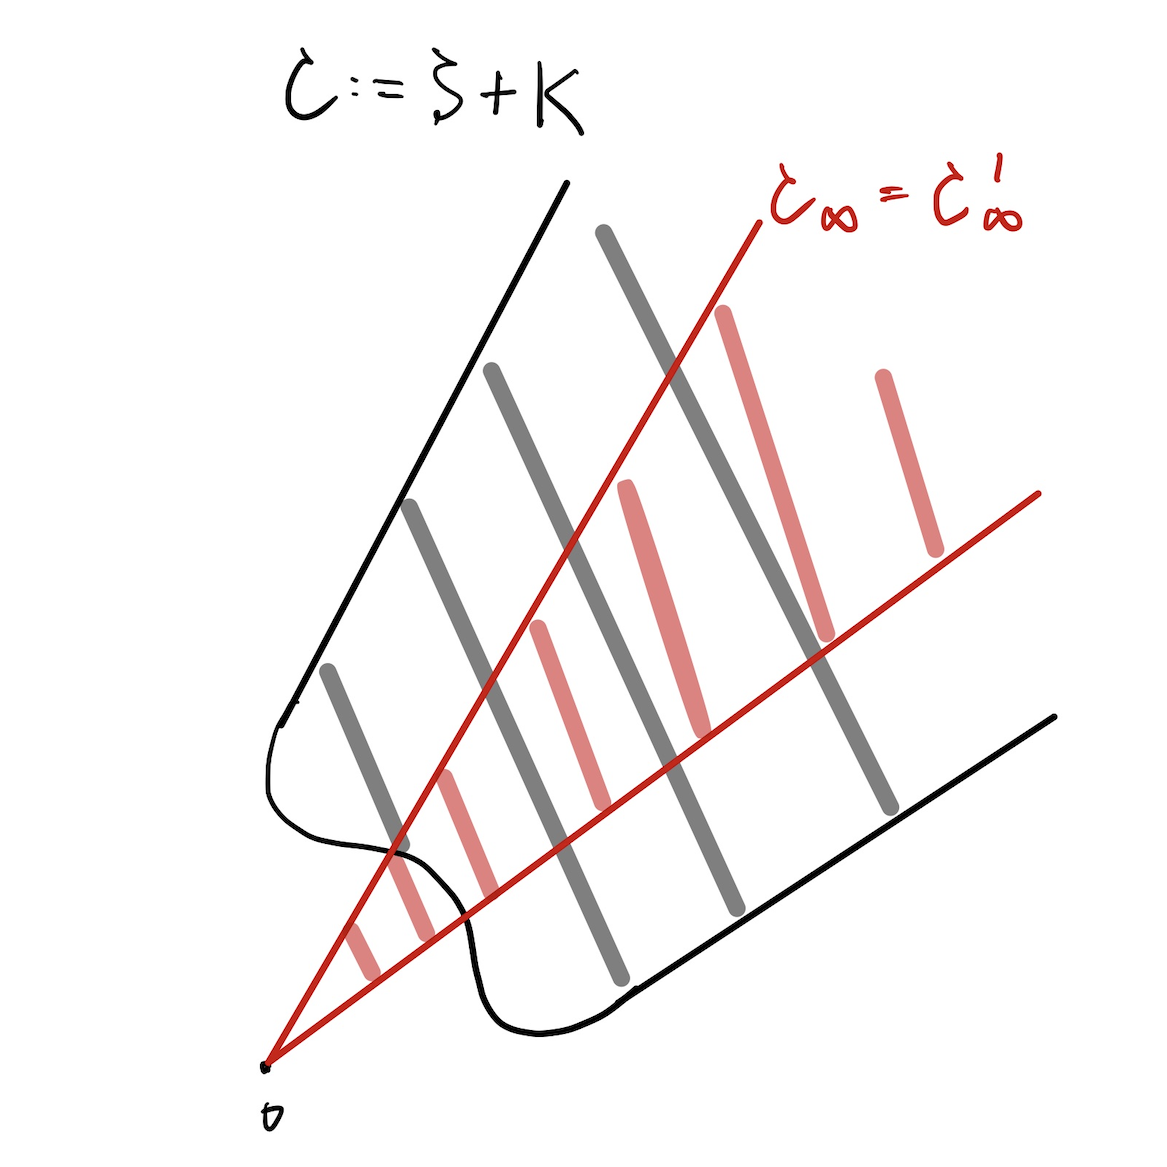
\includegraphics[keepaspectratio, width=40mm]{figures/not_convex_but_asymptotically_regular_3.png}
    \end{center}
    \caption{$C \coloneqq S + K$}
    \label{fig:three}
  \end{minipage}
\end{figure}

\begin{proof}
  We show that for any $d \in C_{\infty}$, $d \in C_{\infty}^1$.

  By the definition of the asymptotic cone,

  \begin{equation}
    \exists t_k \rightarrow \infty, \exists x_k \in C \:\text{with}\: \lim_{k \to \infty} \frac{x_k}{t_k} = d. \notag
  \end{equation}

  As $S$ is compact, $S$ is asymptotically regular, that is,

  \begin{equation}
    \forall t'_l \rightarrow \infty, \exists s_l \in C \:\text{with}\: \lim_{l \to \infty} \frac{x_l}{t'_l} = 0. \notag
  \end{equation}

  For each $k$,

  \begin{equation}
    \exists s_k \in S, b_k \in K \SuchThat x_k = s_k + b_k. \notag
  \end{equation}

  Then we get $d \in k_{\infty}$ because it holds that

  \begin{equation}
    \exists t_k \rightarrow \infty, \exists b_k \in K \:\text{with}\: \frac{b_k}{t_k} \rightarrow d. \notag
  \end{equation}

  The convexity of $K$ and Proposition 2.1.3 lead to $d \in K_{\infty}^1$.

  Thus we obtain $d \in C_{\infty}^1$ because it holds that

  \begin{equation}
    \forall t'_l \rightarrow \infty, \exists x_l \in C \:\text{where}\: x_l \coloneqq b_l + s_l \:\text{with}\: \lim_{l \to \infty} \frac{x_l}{t'_l} = d. \notag
  \end{equation}

  Therefore $C_{\infty} = C_{\infty}^1$.

\end{proof}

\REMARK{2.1.1}{
  Note that the definitions of $C_{\infty}$ and $C_{\infty}^1$ are related to the theory of set convergence of Painleve-Kuratowski. Indeed, for a family $\{C_t\}_{t>0}$ of subsets of $\NDemenstionalRealEuclidianSpace$, the outer limit as $t \rightarrow + \infty$ is the set.

  \begin{equation}
    \limsup_{t \to +\infty} C_t = \{x \:|\: \liminf_{t \to +\infty} d(x, C_t) = 0\}, \notag
  \end{equation}

  while the inner limit as $t \rightarrow +\infty$ is the set

  \begin{equation}
    \liminf_{t \to +\infty} C_t = \{x \:|\: \limsup_{t \to +\infty} d(x, C_t) = 0\}, \notag
  \end{equation}

  It can then be verified that the corresponding asymptotic cones can be written as

  \begin{equation}
    C_{\infty} = \limsup_{t \to +\infty} t^{-1} C,\:\: C_{\infty}^1  = \liminf_{t \to +\infty} t^{-1} C. \notag
  \end{equation}
}

\PROPOSITION{}{
  Let $\{C_t\}_{t > 0}$, $C \subset \NDemenstionalRealEuclidianSpace$, and $C \ne \varnothing $. Then,

  \begin{enumerate}
    \item $C_{\infty} = \limsup_{t \to + \infty} t^{-1}C$, and
    \item $C_{\infty}^{1} = \liminf_{t \to + \infty} t^{-1}C$.
  \end{enumerate}
}

\begin{proof}
  First, we show that (i).

  \begin{enumerate}[label=i-\alph*,align=CenterWithParen]
      \item We prove $C_{\infty} \subset \limsup_{t \to + \infty} t^{-1}C$.

      $\forall d \in C_{\infty}$,

      \begin{equation}
        \exists t_k \rightarrow \infty, \exists x_k \in C \:\text{with}\: \lim_{k \to \infty} \frac{x_k}{t_k} = d. \notag
      \end{equation}

      In other words, it holds that

      \begin{equation}
        \forall \epsilon > 0, \exists k_0 \in \NaturalNumberSet \SuchThat \forall k \geq k_0, \left\lVert \frac{x_k}{t_k} - d\right\rVert < \epsilon. \notag
      \end{equation}

      To obtain $d \in \limsup_{t \to + \infty} t^{-1}C$, we need to show that

      \begin{equation}
        \forall \epsilon > 0, \exists s_0 \in \NaturalNumberSet \SuchThat \forall s \geq s_0, \left\lVert \inf_{u \geq s} \inf_{y \in u^{-1}C} \left\lVert d - y \right\rVert \right\rVert < \epsilon. \notag
      \end{equation}

      To use the assumption of the asymptotic cone, we define a real value

      \begin{equation}
        t(k)_{m} \coloneqq \max \{k, t_{m}\} \:\text{where}\: t_{m} \in \{t_s\}_{s \geq k}^{\infty} \:\text{and}\: m \in \NaturalNumberSet. \notag
      \end{equation}

      Soon we'll get

      \begin{equation}
        \begin{split}
          t(k)_{m} &\geq k, \\
          m &\geq k, \:\text{and}\: \\
          t(k)_{m} &\to \infty \:\text{as}\: m \to \infty. \notag
        \end{split}
      \end{equation}

      Thus $\forall \epsilon > 0, \exists k_0 \in \NaturalNumberSet \SuchThat \forall k \geq k_0,$

      \begin{equation}
        \left\lVert \inf_{u \geq k} \inf_{y \in u^{-1}C} \left\lVert d - y \right\rVert  \right\rVert \leq \inf_{y \in t(k)_{m}^{-1}C} \left\lVert d - y \right\rVert \leq \left\lVert \frac{x_m}{t(k)_{m}} - d \right\rVert < \epsilon. \notag
      \end{equation}

      Then $C_{\infty} \subset \limsup_{t \to + \infty} t^{-1}C$.

      \item We prove $C_{\infty} \supset \limsup_{t \to + \infty} t^{-1}C$.

      We show that $\forall d \in \limsup_{t \to + \infty} t^{-1}C$,

      \begin{equation}
        \exists u_m \to \infty, \exists x_m \in C \:\text{with}\: \lim_{t \to \infty} \frac{x_m}{u_m} = d. \notag
      \end{equation}

      $\forall d \in \limsup_{t \to + \infty} t^{-1}C$, $\forall \epsilon, \exists k_0 \in \NaturalNumberSet \SuchThat \forall k \geq k_0$,

      \begin{equation}
        \left\lVert \inf_{u \geq k} \inf_{y \in u^{-1}C} \left\lVert d - y  \right\rVert  \right\rVert < \frac{\epsilon}{3}. \notag
      \end{equation}

      we let $\alpha(k) \coloneqq \left\lVert \inf_{u \geq k} \inf_{y \in u^{-1}C} \left\lVert d - y  \right\rVert  \right\rVert$. To get $u_{m} \to \infty$ as $m \to \infty$, we define $u_m \coloneqq m$ where $m \geq k$.

      By the definition of infimum, there exist $u_k, \cdots, u_{m_0}, \cdots$ such that

      \begin{equation}
        \begin{split}
          \inf_{y \in u_k^{-1}C} \left\lVert d - y \right\rVert  &< \alpha(k) + \frac{\epsilon}{3}, \\
          &\vdots  \\
          \inf_{y \in u_{m_0}^{-1}C} \left\lVert d - y \right\rVert  &< \alpha(k) + \frac{\epsilon}{3}, \\
          &\vdots. \notag
        \end{split}
      \end{equation}

      Also we let $\beta(m) \coloneqq \inf_{y \in u_m^{-1}C} \left\lVert d - y \right\rVert$ for each $m \geq k$.

      By the definition of infimum, there exist $x_k, \cdots, x_{m_0}, \cdots \in C$ such that

      \begin{equation}
        \begin{split}
          \left\lVert \frac{x_k}{u_k} - d \right\rVert  < \frac{\epsilon}{3} + \beta(k) &< \frac{\epsilon}{3} + \frac{\epsilon}{3} + \alpha(k) = \epsilon, \\
          &\vdots  \\
          \left\lVert \frac{x_{m_0}}{u_{m_0}} - d \right\rVert  < \frac{\epsilon}{3} + \beta(m_0) &< \frac{\epsilon}{3} + \frac{\epsilon}{3} + \alpha(k) = \epsilon, \\
          &\vdots. \notag
        \end{split}
      \end{equation}

      Thus it holds that

      \begin{equation}
        \exists u_m \to \infty, \exists x_m \in C \:\text{with}\: \lim_{t \to \infty} \frac{x_m}{u_m} = d. \notag
      \end{equation}

      Then $C_{\infty} \supset \limsup_{t \to + \infty} t^{-1}C$.

  \end{enumerate}

  Therefore $C_{\infty} = \limsup_{t \to + \infty} t^{-1}C$.

  Second, we show that (ii).

  \begin{enumerate}[label=ii-\alph*,align=CenterWithParen2]
    \item We prove $C_{\infty}^{1} \subset \liminf_{t \to + \infty} t^{-1}C$.

    $\forall d \in C_{\infty}^{1}$,

    \begin{equation}
      \forall t_k \rightarrow \infty, \exists x_k \in C \:\text{with}\: \lim_{k \to \infty} \frac{x_k}{t_k} = d. \notag
    \end{equation}

    Also,

    \begin{equation}
      \forall \epsilon > 0, \exists k_0 \in \NaturalNumberSet \SuchThat \forall k \geq k_0, \left\lVert \frac{x_k}{t_k} - d \right\rVert < \epsilon. \notag
    \end{equation}

    We let $\alpha (s) \coloneqq \sup_{u \geq s} \inf_{y \in u^{-1} C} \left\lVert y - d \right\rVert \geq 0$.z

    For each $s = 1,2,\cdots$, $\exists t_s \geq s$,

    \begin{equation}
      - \frac{1}{s} \leq \alpha (s) - \frac{1}{s} < \inf_{y \in t_{s}^{-1} C} \left\lVert y - d \right\rVert \leq \left\lVert \frac{x_s}{t_s} - d \right\rVert. \notag
    \end{equation}

    Now $\{t_k\}_{k \in \NaturalNumberSet}$ satisfies $t_k \to \infty$.

    Since $d \in C_{\infty}^{1}$,

    \begin{equation}
      \exists x_s \in C \SuchThat \lim_{k \to \infty} \frac{x_s}{t_s} = d. \notag
    \end{equation}

    Thus $d \in \liminf_{t \to + \infty} t^{-1}C$.

    \item We prove $C_{\infty}^{1} \supset \liminf_{t \to + \infty} t^{-1}C$.

    $\forall d \in \liminf_{t \to + \infty} t^{-1}C$,

    \begin{equation}
      \forall \epsilon, \exists s_0 \in \NaturalNumberSet \SuchThat \forall s \geq s_0, 0 \leq \sup_{u \geq s} \inf_{y \in u^{-1} C} \left\lVert y - d \right\rVert < \epsilon. \notag
    \end{equation}

    $\forall n \geq s$,

    \begin{equation}
      0 \leq \inf_{y \in n^{-1}C} \left\lVert y - d \right\rVert \leq \sup_{u \geq s} \inf_{y \in u^{-1} C} \left\lVert y - d \right\rVert < \epsilon. \notag
    \end{equation}

    By the definition of infimum, for any $\{t_k\} \to \infty$,

    \begin{equation}
      \exists u_0 \geq s \:\text{where}\: t_{u_0} \geq s \SuchThat \forall u \geq u_0, \exists x_u \in C, \left\lVert \frac{x_u}{t_u} - d \right\rVert < \epsilon. \notag
    \end{equation}

    Thus $d \in C_{\infty}^{1}$.

  \end{enumerate}

  Therefore $C_{\infty}^{1} = \liminf_{t \to + \infty} t^{-1}C$.
\end{proof}

\PROPOSITION{2.1.4}{
  Let $C \subset \NDemenstionalRealEuclidianSpace$ be nonempty and define the normalized sets.

  \begin{equation}
    C_N \coloneqq \{d \in \NDemenstionalRealEuclidianSpace \:|\: \exists \{x_k\} \in C, \left\lVert x_k \right\rVert \rightarrow +\infty \:\text{with}\: d = \lim_{k \to \infty} \frac{x_k}{\left\lVert x_k \right\rVert }\}. \notag
  \end{equation}

  Then $C_{\infty} = \text{pos}\:C_N$, where for any set $C$, $\text{pos}\:C = \{\lambda x \:|\: x \in C, \lambda \geq 0\}$.
}

\begin{proof}
  Clearly, one always has $\text{pos}\:C_N \subset C_{\infty}$. Conversely, let $0 \ne d \in C_{\infty}$.

  Then there exists $t_k \rightarrow \infty$, $x_k \in C$ such that

  \begin{equation}
    d = \lim_{k \to \infty} \frac{x_k}{t_k} = \lim_{k \to \infty} \frac{1}{t_k} \cdot \left\lVert x_k \right\rVert \cdot \frac{x_k}{\left\lVert x_k \right\rVert }, \:\text{with}\: \left\lVert x_k \right\rVert \rightarrow \infty. \notag
  \end{equation}

  Thus the sequence $\{t_k^{-1}\left\lVert x_k \right\rVert \}$ is a nonnegative bounded sequence, and by the Bolzano-Weierstrass theorem, there exists a subsequence $\{t_k^{-1}\left\lVert x_k \right\rVert\}_{k \in K}$ with $K \subset \NaturalNumberSet$ such that $\lim_{k \in K} t_k^{-1} \left\lVert x_k \right\rVert = \lambda \geq 0$, which means that $d = \lambda d_N$ with $d_N \in C_N$, namely $d \in \text{pos}\:C_N$.
\end{proof}

\PROPOSITION{2.1.5}{
  Let $C$ be a nonempty convex set in $\NDemenstionalRealEuclidianSpace$. Then the asymptotic cone $C_{\infty}$ is a closed convex cone. Moreover, define the following sets:
  \begin{equation}
    \begin{split}
      D(x) &\coloneqq \{d \in \NDemenstionalRealEuclidianSpace \:|\: x + td \in \text{cl}\:C, \forall t >0\}\: \forall x \in C, \\
      E &\coloneqq \{d \in \NDemenstionalRealEuclidianSpace \:|\: \exists x \in C \SuchThat x + td \in \text{cl}\:C, \forall t > 0\}, \\
      F &\coloneqq \{d \in \NDemenstionalRealEuclidianSpace \:|\: d + \text{cl}\:C \subset \text{cl}\:C\}. \notag
    \end{split}
  \end{equation}

  Then $D(x)$ is in fact independent of $x$, which is thus now denoted by $D$, and $C_{\infty} = D = E = F$.
}

\begin{proof}
  We show that

  \begin{enumerate}[label=\roman*,align=CenterWithParen]
    \item $C_{\infty}$ is convex,
    \item $C_{\infty} \subset D(x)$,
    \item $D(x) \subset E$,
    \item $E \subset C_{\infty}$,
    \item $C_{\infty} \subset F$,
    \item $C_{\infty} \supset F$.
  \end{enumerate}

  \begin{enumerate}[label=\roman*,align=CenterWithParen]
    \item We'll show that $C_{\infty}$ is convex.

    It follows that $C$ is asymptotically regular from Proposition 2.1.3.

    For any $d_1$ and $d_2$,

    \begin{equation}
      \begin{split}
        \forall t_k &\rightarrow \infty, \exists \{x_k\}_{k=1}^{\infty} \:\text{with}\: \frac{x_k}{t_k} \rightarrow d_1 \:\text{as}\: k \rightarrow \infty \\
        (\forall \epsilon &> 0, \exists k_0 \in \NaturalNumberSet \SuchThat \forall k \geq k_0, \left\lVert \frac{x_k}{t_k} - d_1\right\rVert < \epsilon ), \\
        \forall s_l &\rightarrow \infty, \exists \{y_l\}_{l=1}^{\infty} \:\text{with}\: \frac{y_l}{s_l} \rightarrow d_2 \:\text{as}\: l \rightarrow \infty \\
        (\forall \epsilon &> 0, \exists l_0 \in \NaturalNumberSet \SuchThat \forall l \geq l_0, \left\lVert \frac{y_l}{s_l} - d_2\right\rVert < \epsilon ). \notag
      \end{split}
    \end{equation}

    Then we'll check the convexity, that is,

    \begin{equation}
      \lambda d_1 + (1 - \lambda) d_2 \in C_{\infty} \:\text{where}\: \lambda \in (0,1). \notag
    \end{equation}

    We take a sequence $\{u_m\}_{m=1}^{\infty}$ where $u_m \coloneqq \max \{t_m,s_m\}$ and $m_0 \coloneqq \max \{k_0,l_0\} \in \NaturalNumberSet$.

    Then you can find $u_m \rightarrow \infty$.

    Also we define a sequence as $\{ \lambda x_m + (1 - \lambda) y_m \}_{m=1}^{\infty}$.

    $\forall m \geq m_0$,

    \begin{equation}
      \begin{split}
        \left\lVert \frac{\lambda x_m + (1 - \lambda) y_m}{u_m} - (\lambda d_1 + (1 - \lambda) d_2) \right\rVert &\leq \lambda \left\lVert \frac{x_m}{u_m} - d_1 \right\rVert + (1 - \lambda) \left\lVert \frac{y_m}{u_m} - d_2 \right\rVert \\
        &< \lambda \epsilon + (1 - \lambda) \epsilon = \epsilon. \notag
      \end{split}
    \end{equation}

    Therefore $C_{\infty}$ is convex.

    \item We now prove that $C_{\infty} \subset D(x)$

  \end{enumerate}
\end{proof}
\end{document}
